\documentclass[a4paper]{article}

%%%%%%%%%%%%%%%%%%%%%%%%%%%%%%%%%% 
% Package for making LaTeX properly handle utf8 characters set and danish language rules
\usepackage[utf8]{inputenc}
\usepackage[danish]{babel}

%%%%%%%%%%%%%%%%%%%%%%%%%%%%%%%%%% 
% Package for changing to a nicer font 
\usepackage[T1]{fontenc}

%%%%%%%%%%%%%%%%%%%%%%%%%%%%%%%%%% 
% Package for conctroling the text area
\usepackage[margin=2.5cm]{geometry}

%%%%%%%%%%%%%%%%%%%%%%%%%%%%%%%%%% 
% Package for inserting clickable hyperlinks in pdf versions as produced by pdflatex
\usepackage{enumitem, hyperref}

%%%%%%%%%%%%%%%%%%%%%%%%%%%%%%%%%% 
% Package for including figures. TeX and thus LaTeX was developped before the existence of directory file-structures, but the graphicspath let's you add directories, that the \includegraphics will search.
\usepackage{graphicx}
\graphicspath{{figures/}}

%%%%%%%%%%%%%%%%%%%%%%%%%%%%%%%%%% 
% Package for typesetting programs. Listings does not support fsharp, but a little modification goes a long way
\usepackage{listings}
\usepackage{xcolor}
\usepackage{verbatim}
\usepackage{color}


\renewcommand{\figurename}{Figur}
\renewcommand{\contentsname}{Indholdsfortegnelse}
\renewcommand{\contentsname}{Table of Contents}
\renewcommand{\lstlistingname}{Kildekode}
\renewcommand{\partname}{Afsnit}

\def\sectionautorefname~#1\null{%
  Afsnit #1\null
}

\def\subsectionautorefname~#1\null{%
  Afsnit #1\null
}

\def\figureautorefname~#1\null{%
  Figur #1\null
}

\def\equationautorefname~#1\null{%
  Ligning #1\null
}

\def\namedlabel#1#2{\begingroup
    #2%
    \def\@currentlabel{#2}%
    \phantomsection\label{#1}\endgroup
}

\definecolor{bluekeywords}{rgb}{0.13,0.13,1}
\definecolor{greencomments}{rgb}{0,0.5,0}
\definecolor{turqusnumbers}{rgb}{0.17,0.57,0.69}
\definecolor{redstrings}{rgb}{0.5,0,0}
\definecolor{lightgray}{RGB}{240, 240, 240}

\newcommand{\namedref}[1]{\autoref{#1} - \nameref{#1} på Side \pageref{#1}}

\lstdefinelanguage{FSharp}
				{morekeywords={\#load, \#r, let, new, match, with, rec, open, module, namespace, type, of, member, and, for, in, do, begin, end, fun, function, try, mutable, if, then, else, List, Set, Sudoku, Seq, false, true, Assert, printfn, print, sprintf, when, ->, >, ::, printf, yield, this},
	keywordstyle=\color{bluekeywords},
	sensitive=false,
	morecomment=[l][\color{greencomments}]{///},
	morecomment=[l][\color{greencomments}]{//},
	morecomment=[s][\color{greencomments}]{{(*}{*)}},
	morestring=[b]",
	stringstyle=\color{redstrings},
	tabsize=2, % sets default tabsize to 2 spaces
	backgroundcolor=\color{lightgray}
}

\usepackage[table]{}
\usepackage{array}
\usepackage{algorithm}
\usepackage{caption}
\usepackage{float}
\usepackage{amsmath}
\usepackage{algorithm}
\usepackage[noend]{algpseudocode}
\usepackage{mathtools}
\usepackage{ragged2e}
\usepackage{caption}
\usepackage{amssymb}
\usepackage{nameref}
\usepackage{lmodern}

\lstset{ %
  numbers=right,                    % where to put the line-numbers; possible values are (none, left, right)
  numbersep=5pt,                   % how far the line-numbers are from the code
  numberstyle=\small\color{bluekeywords}, % the style that is used for the line-numbers
  stepnumber=1,                    % the step between two line-numbers. If it's 1, each line will be numbered
  title=\lstname,                   % show the filename of files included with \lstinputlisting; also try caption instead of title
  showstringspaces=false,
  breaklines=true,
  captionpos=b,
  language=FSharp,
  texcl=true,
  extendedchars=true,
  inputencoding=utf8
  }

\setlength\parindent{0pt}

%%%%%%%%%%%%%%%%%%%%%%%%%%%%%%%%%%
% Package or using suits
\usepackage{kmath,kerkis}
\normalfont

\usepackage{fancyhdr}
\usepackage{lastpage}
 
\pagestyle{fancy}
\fancyhf{}
 
\rhead{Mads U. Svendsen, Anders F. Jørgensen, Nicolai L. Hargreave, Bo H. Thomsen}
\rfoot{Side \thepage \hspace{1pt} af \pageref{LastPage}}

\title{Prey \& The Predators - Programmering og Problemløsning}
\author{Mads U. Svendsen, Anders F. Jørgensen, Nicolai L. Hargreave, Bo H. Thomsen}

\begin{document}
	\maketitle
  \tableofcontents
\section{Forord}
  Denne opgave er lavet i Programmering og Problemløsning(PoP),
    på Datalogisk Institut - Københavns Universitet(DIKU) - første semester år 2015/2016.
    Opgaven har opgavenummeret 11g.
    I gruppen er Mads U. Svendsen, Anders F. Jørgensen, Nicolai L. Hargreave og Bo H. Thomsen.
\newpage
    
\section{Introduktion} \label{sec:introduction}
   I dette projekt er målet at udvikle en simulator,
   den kan simulere det kendte Prey/Predator udviklings problem.
   Simulatoren skal vise udviklingen blandt en gruppe af byttedur, 
   og en gruppe af rovdyr. Hvordan mængden af rovdyr i perioder stiger,
   men når de så når et specielt sted - falder kraftigt. Hvorefter mængden af byttedyr stiger.
   Målet for projektet er at vende sig til objekter, klasser, abstrakte klasser og inheritance.

  \paragraph*{Sådan kompilerer du projektet\\}
    I \path{/src} mappen ligger \path{simulation.fsx},
    den kan kompileres med fsharpc og køres med mono.
    Den generere \path{simulation.exe}.

    Tests findes i  mappen \path{/src}, i filen \path{test.fsx}.

\section{Problemformulering} \label{sec:problem}
  Vi vil i dette projekt, bygge en ssimulator der kan simulere,
  hvordan flere arter lever sammen i et hapitat.
  Når nogle typer har den egenskab, at de kan spise andre.
  I dette eksempel operere vi kun med to typer dyr, "Prey" og "Predator".

  \subsection{Kravspecifikation} \label{ssec:demands}
    
  \section{Problemanalyse og design} \label{sec:design}
    Efter at vi havde deffineret kravene til vores produkt(Se \namedref{ssec:demands}),
    satte vi os ned og opbyggede en klasse struktur.
    Voers ide til strukturen kan ses i \namedref{fig:umlDiagram}.

    \begin{figure}[H]
      \centering

      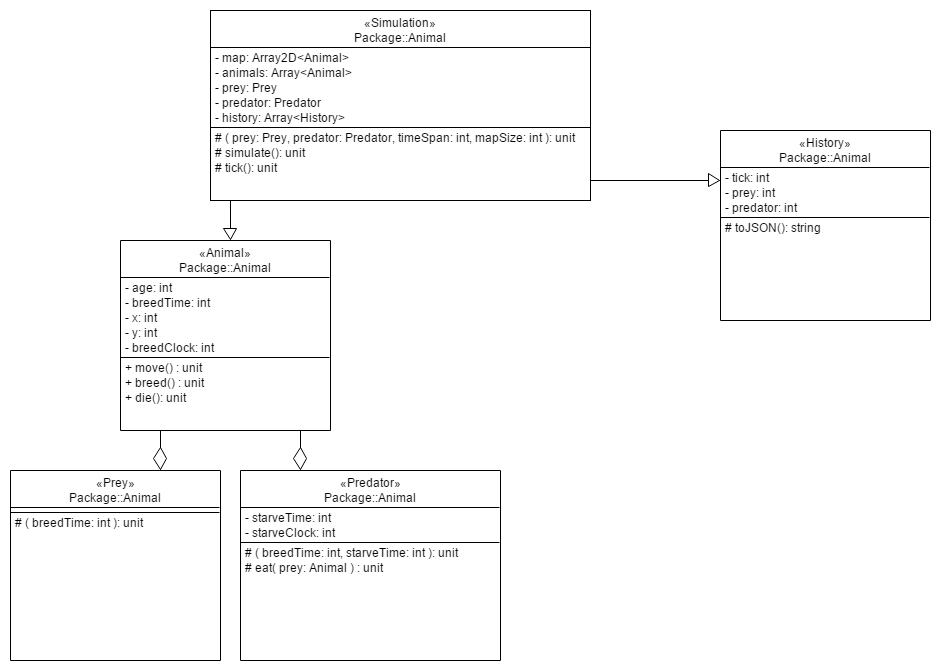
\includegraphics[width=520px]{figures/uml.png}

      \caption{UML diagram over vores klasse design}
      \label{fig:umlDiagram}
    \end{figure}

    Vi har haft flere overvejeler omkring det med starttilstand/indstillinger.
    Efter snakken frem og tilbage mellem kommandopropt-input og filbaseret input,
    er vi kommet frem til at bruge en fil.
    Det giver os den reneste kode og giver nem mulighed for at tilføje flere indstillinger.
    Filformatet for denne fil kunne være flere, både ".csv", ".txt" og "json" er gode formater,
    de to første er meget simple, mens ".json" er meget struktureret og det sikre en hvis datastruktur
    og mulighed for bedre error tjek. Derfor er valget faldet på ".json".

    Omkring output fil har vi også snakket om flere filformater,
    ".csv" er et meget bredt brugt format til simulationsdata,
    mens ".json" er nemt at læse ind fra. ".json" giver mest struktur,
    og afspejler også vores interne design og derfor faldt valget på det.

    \subsection*{Simulation}

    \subsection*{Animal}

      \subsubsection*{Prey}

      \subsubsection*{Predator}

    \subsection*{Settings}
      Typen \texttt{Settings} er et container element, 
      der indeholder starttilstanden for simulationen.
      Den giver en struktureret måde at gemme og tilgå de indstilliger der skal bruges.
      For at al logikken omkring indstillinger er indeholdt i en klasse,
      har vi valgt at klassen også selv loader en fil.

      Et Settings objekt kan derfor heller ikke oprettes uden at der gives en fil.

    \subsection*{HistoryRecord}
      HistoryRecord er en container klasse, der indeholder tilstanden for habitatet efter et tick.
      Den skal indeholde antal ticks siden start, antal preys og antal predators ved dette tick.
      Denne klasse ligger så struktur for et element i den JSON fil der gemmes når simulationen er slut.

  \section{Programbeskrivelse} \label{sec:programDescription}
    
      
  \section{Afprøvning} \label{sec:unitTest}
    

	\section{Diskussion og konlusion} \label{sec:conclusion}
   
  \section{Bilag}
     
      \subsection{Brugervejledning} \label{ssec:manual}
        
      \subsection{Kildekode} \label{ssec:sourceCode}
        
        \lstinputlisting[caption={Simulations klasser},label={lst:classes}]{../src/classes.fsx}
        \lstinputlisting[caption={Simulations klasser},label={lst:simulation}]{../src/simulation.fsx}
        \lstinputlisting[caption={Simulations klasser},label={lst:test}]{../src/test.fsx}

      \subsection{Billeder}
        
\end{document}